% !TEX TS-program = pdflatex
% !TEX encoding = UTF-8 Unicode


\documentclass[11pt]{article}
\usepackage[utf8]{inputenc}

%%% PAGE DIMENSIONS
\usepackage{geometry}
\geometry{letterpaper}
\geometry{margin=1in} % for example, change the margins to 2 inches all round

\usepackage{graphicx} % support the \includegraphics command and options
\usepackage[parfill]{parskip} % Activate to begin paragraphs with an empty line rather than an indent

%%% HEADERS & FOOTERS
\usepackage{fancyhdr} % This should be set AFTER setting up the page geometry
\pagestyle{fancy} % options: empty , plain , fancy
\renewcommand{\headrulewidth}{0pt} % customise the layout...
\lhead{}\chead{}\rhead{}
\lfoot{}\cfoot{\thepage}\rfoot{}

%%% SECTION TITLE APPEARANCE
\usepackage{sectsty}
\allsectionsfont{\sffamily\mdseries\upshape}
% (See the fntguide.pdf for font help)
% (This matches ConTeXt defaults)

%%% END Article customizations

\title{Slow Earthquakes: A Manifestation of Transitional Frictional Behavior}
\author{J.R. Leeman, D.M. Saffer, C. Marone}
\date{} % Activate to display a given date or no date (if empty),
         % otherwise the current date is printed

\bibliographystyle{unsrt}

\begin{document}
\maketitle

\section{Introduction}
Observations of slow-slip and low-frequency earthquakes in nature suggest that
fault failure encompasses a spectrum of slip modes \cite{Peng:2010, Ide:2007,
Beroza:2011}.  While the explanations for non-traditional earthquakes remain a
topic of debate, they have been observed in many subduction zones, including
Cascadia \cite{Miller:2002, Rogers:2003}, Mexico \cite{Kostoglodov:2003}, Costa
Rica \cite{Jiang:2012}, Japan \cite{Ito:2006}, and New Zealand
\cite{Wallace:2010}. What causes strain energy to be released across a
wide-range of failure behaviors is not well understood, but transitional
frictional stability is a  possible explanation. System stability is defined in
terms of stiffness as $k \sim k_{critical}$ \cite{Gu:1984} and can be altered by
environmental variables such as effective normal stress, critical slip distance,
and the velocity dependence of friction. Clustering of slow and transitional
events around traditional seismic faults in nature suggests that transitional
behavior is responsible. Laboratory evidence of this behavior is scattered
\cite{Kaproth:2013, Baumberger:1994, Leeman:2015}, mostly suggested by numerical
models \cite{Gu:1984}. Here we present the first systematic investigation of the
critical stiffness ratio and its effect on the frictional state of a laboratory
fault. We also show that stiffness can control the slip mode and that the
failure mode can change as stiffness is influenced by accumulated fault slip and
damage zone evolution.  


\section{Main}
Biaxial double-direct shearing experiments were performed with humidified
Min-U-Sil\textsuperscript{\textregistered} simulated fault gouge. Force and
displacement are recorded on both the normal and shear axes, as well as a measurement of the shearing
block position (Fig.\ref{Fig:Biax Schematic}). System compliance can be modified
by changing the normal stress (2,4,6,8,12 MPa) or the material of which the
central shearing block is made (steel or cast acrylic).

% Figure %
\begin{figure}
    \centering
    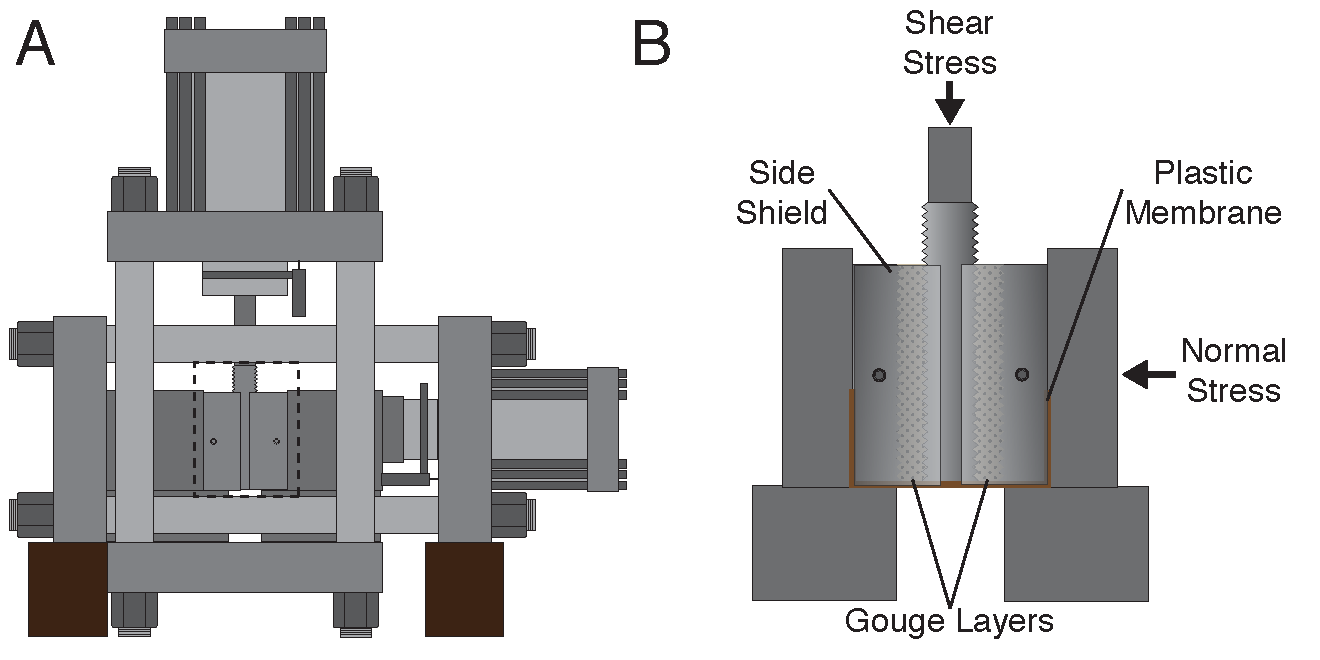
\includegraphics[scale=0.5]{../Figures/Fig_Biax_Schematic/biax_schematic.pdf}
       \caption{The biaxial deformation apparatus (A) and sample configuration (B).
       Two large hydraulic pistons are servo-controlled in either force or
       displacement control modes. Double direct shear samples are supported by
       steel blocks. Samples use metal side shields and a plastic membrane to
       reduce gouge extrusion.  Local displacement transducers (DCDTs) can be
       referenced to the center block to avoid apparatus stiffness effects on
       the measurement.}
      \label{Fig:Biax Schematic}
\end{figure}
% End Figure %

For experiments exhibiting stable sliding behavior, velocity steps were imposed
to obtain the rate-and-state frictional parameters of the material and system.
The rate-and-state parameters are constants to an empirical fit to transient
response of a frictional system to a perturbation \cite{Marone:1998,Dieterich:1979,Ruina:1983}. The $a$
parameter provides a measure of the direct effect in response to a velocity
step, and $b$ provides the magnitude of friction evolution there-after. The
difference of $a$ and $b$, then yields a quantitative measure of how strongly
velocity strengthening or velocity weakening a material is. The critical slip
distance, $D_c$, is often considered to be the slip required to renew the
contact population in a granular material. In our experiments, $a$ remains
relatively constant with displacement, but $b$ evolves asymptotically upwards
with increasing shear displacement. During this transitional period, the
critical slip distance evolves downwards (Fig.\ref{Figure:RSF Props}).

% Figure %
\begin{figure}
    \centering
        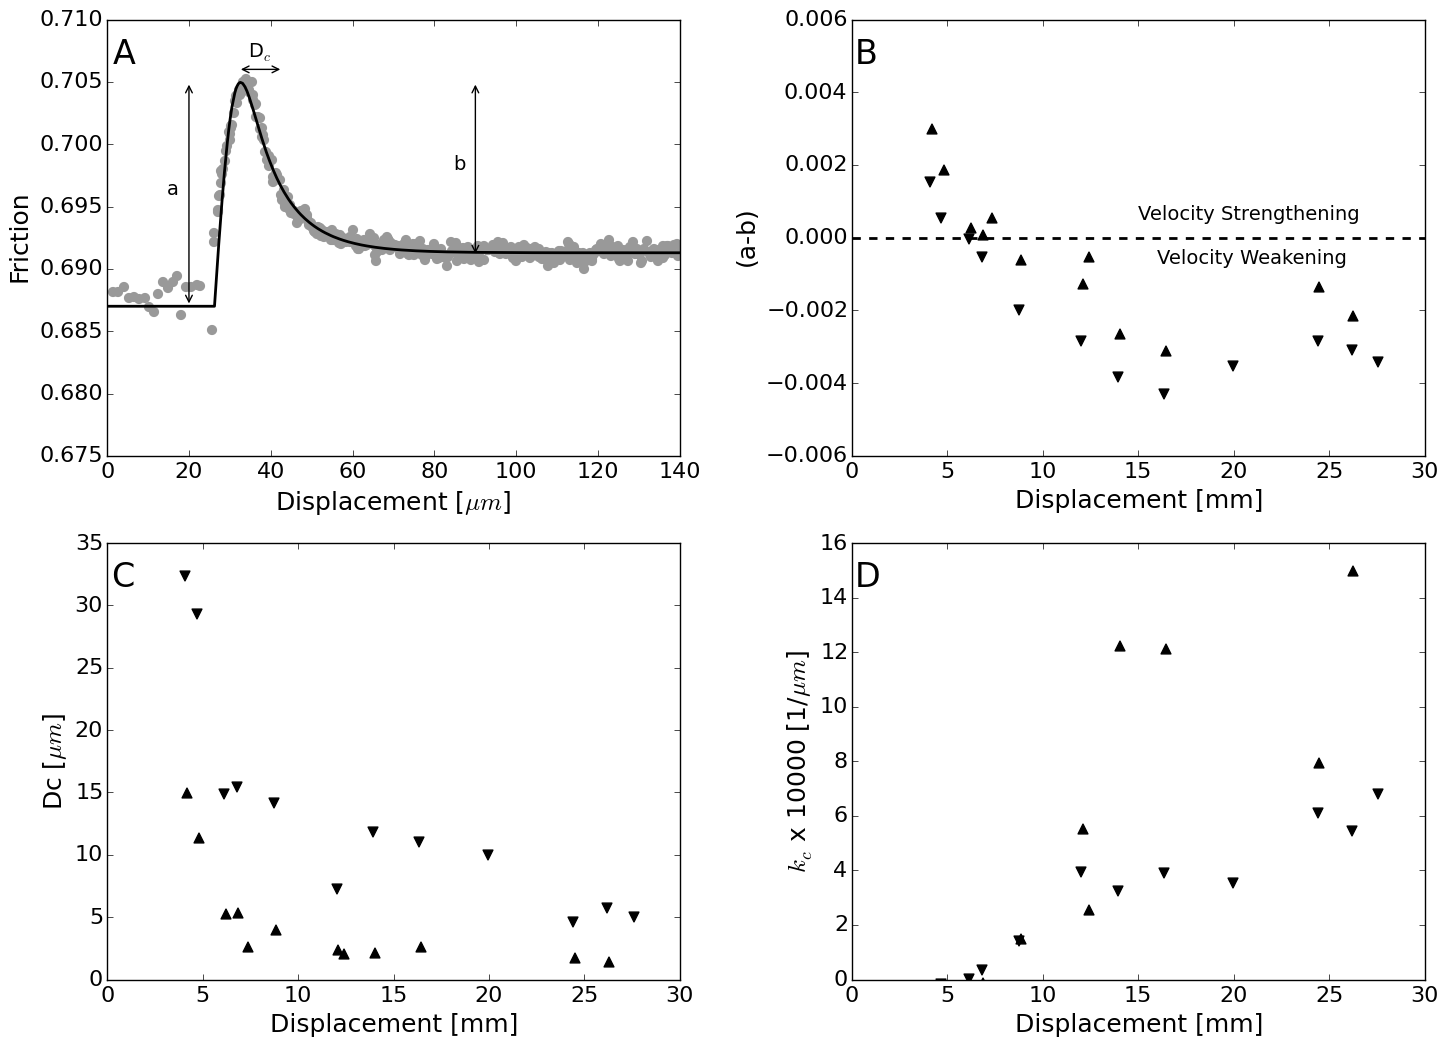
\includegraphics[scale=0.45]{../Figures/Fig_RSF_Parameters/RSF_Parameters.png}
       \caption{Rate-and-state friction parameters obtained from velocity step
       inversions. All inversions were accomplished with a fixed stiffness of
       $k=$5.5x$10 ^ {-3} \mu$m. A) rate-and-state parameter $a$ remains relatively
       constant with displacement and shows a systematic behavior with higher
       values of $a$ always being observed during velocity up-steps. The $b$
       parameter shows a similar behavior, but also increases with displacement,
       reaching a steady-state value $\sim$10 mm displacement. B) The sample
       transitions from velocity strengthening to velocity weakening  behavior
       at $\sim$10 mm and remains velocity weakening for the remainder of  the
       experiment. C) Critical slip distance estimates show considerable
       scatter,  but do reduce to a steady-state value of 5-10 um.}
      \label{Figure:RSF Props}
\end{figure}
% End Figure %

There are two conditions for unstable behavior to occur: 1) that the material be
velocity neutral to velocity weakening, and 2) that the system stiffness be at
or below the critical stiffness \cite{Marone:1998, Scholz:2002}. Velocity
weakening is a necessary, but insufficient condition for unstable behavior. If a
material is velocity strengthening, any acceleration leading to slip is
immediately arrested by increased shearing resistance and the energy is
frictionally dissipated. The stiffness of the system governs the rate at which
energy stored as strain can be released. If the energy release occurs in such a
way that the drop in shear resistance with displacement occurs faster than the
drop in applied shearing force with displacement, the system can support
unstable failure.

In a stiff (all steel) forcing setup, linearly stable frictional behavior was observed.
In a more compliant loading system, emergent unstable behavior was observed.
Unstable behavior began with frictional oscillations, transitioning to dynamic frictional
failure. Oscillations and dynamic failure are characterized by relatively rapid
accelerations and decelerations of the system above/below the load point
velocity when the material yields under excessive shear force. Experiments with
further increased compliance, rapid dynamic failure was observed. These events
were audible and classified as fast stick-slip.

The system stiffness was measured, for both stable and unstable experiments, with
cycles of unloading and reloading the shear stress at a constant displacement rate of $10 \mu m/s$.  This provided an estimate
of the aggregate system shear stiffness. For experiments that became unstable,
a second method of stiffness measurement was employed. Loading stiffnesses of
individual slip events were algorithmically determined \cite{Leeman:2015}. We expect both
of these methods to provide comparable results and allow determination the system's behavior.

In both determinations of stiffness, we observe increases in measured aggregate
system stiffness with accumulated shearing displacement. Unload/reload measurements show these increases are most
prevalent in the first 10 mm of shear, asymptotically approaching steady-state.
Initial increases in stiffness could be due to layer compaction from
grain rearrangement, layer thinning with increased shear strain, grain
comminution, localization of shear, or reduction of
compliant center block material above the sample due to geometric effects.
Layer compaction due to rearrangement and geometric thinning with shear
have been well documented \cite{Scott:1994}.  At these low stresses, grain
comminution is minimal. Shear localization effects have been shown to play a role in the
evolution of layer behavior \cite{Logan:1992}, especially before reaching mechanical
steady-state as R and Y shears develop. The reduction in the amount of
compliant center block material above the shearing zone with accumulated
displacement is minimal compared to these other effects.

Stiffnesses recovered from the loading portion of individual stick-slip events
is lower than that from unload/reloads at low displacements. These low values
of “working stiffness” do not represent the overall stiffness of the system, but
a stiffness influenced by continued slip and creep. As dynamic failure reaches a
steady state, we see agreement between the two methods of stiffness measurement
(Fig.\ref{Figure:Stiffness Methods}).

% Figure %
\begin{figure}
    \centering
        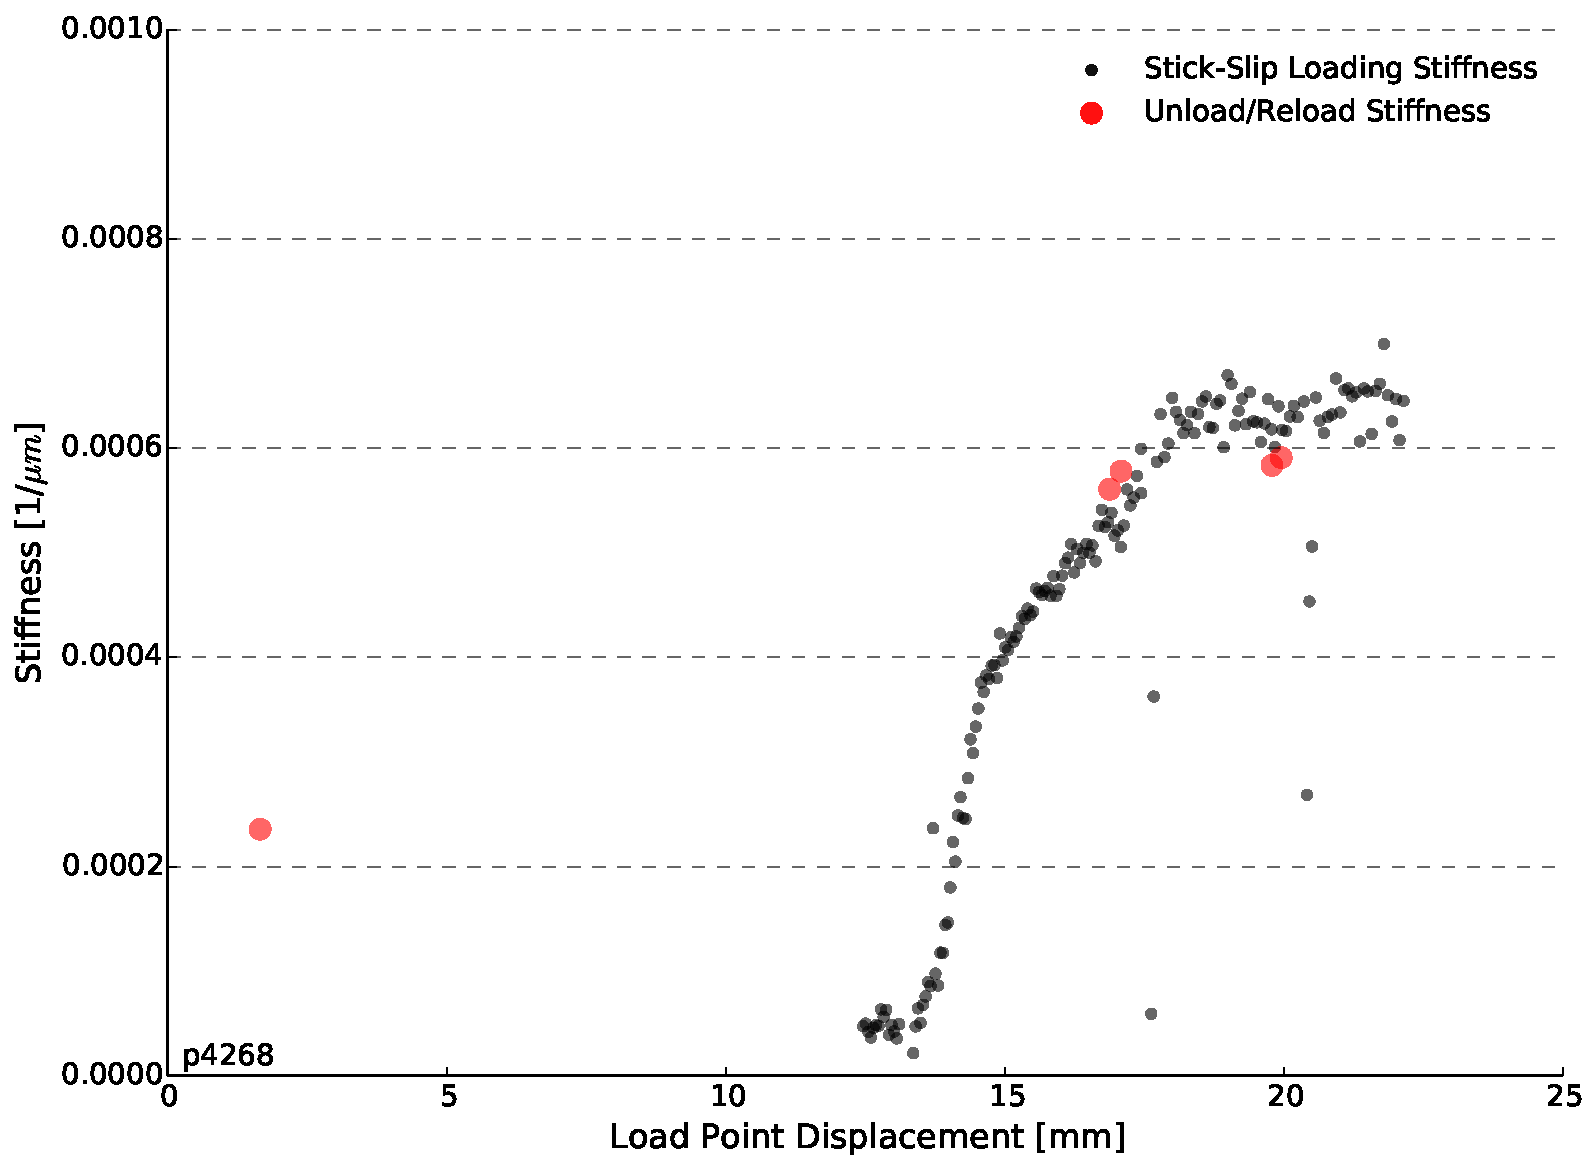
\includegraphics[scale=0.4]{../Figures/Fig_Stiffness_Methods/Stiffness_Methods.pdf}
       \caption{When the sytem is at steady-state, the two methods of stiffness
       estimation provide comparable results. At low displacements, early stick-slip
       events appear more compliant than bulk system measurements. This is due to the
       not fully dynamic failure of the events and creep during the loading phase.}
      \label{Figure:Stiffness Methods}
\end{figure}
% End Figure %

The transition from velocity strengthening to velocity weakening and
corresponding decrease in $D_c$ increase the value of the predicted critical
stiffness (eq.\ref{equation:kc}). Combined with increasing system stiffness,
a frictional transition is predicted as the critical stiffness intersects the
measured system stiffness. We begin to see frictional oscillations and dynamic
failure as $k \sim k_c$. The larger the departure from $k=k_c$, the more dramatic the behavior.
Very compliant systems exhibit fast dynamic failure. Very stiff systems show no
tendency to produced damped oscillations after a
velocity step (Fig.\ref{Figure:Runplot}).

% Equation - Critical Stiffness %
\begin{equation}
    k_c = \frac{b-a}{D_c}
	\label{equation:kc}
\end{equation}
% End Equation %

% Figure %
\begin{figure}
	\centering
		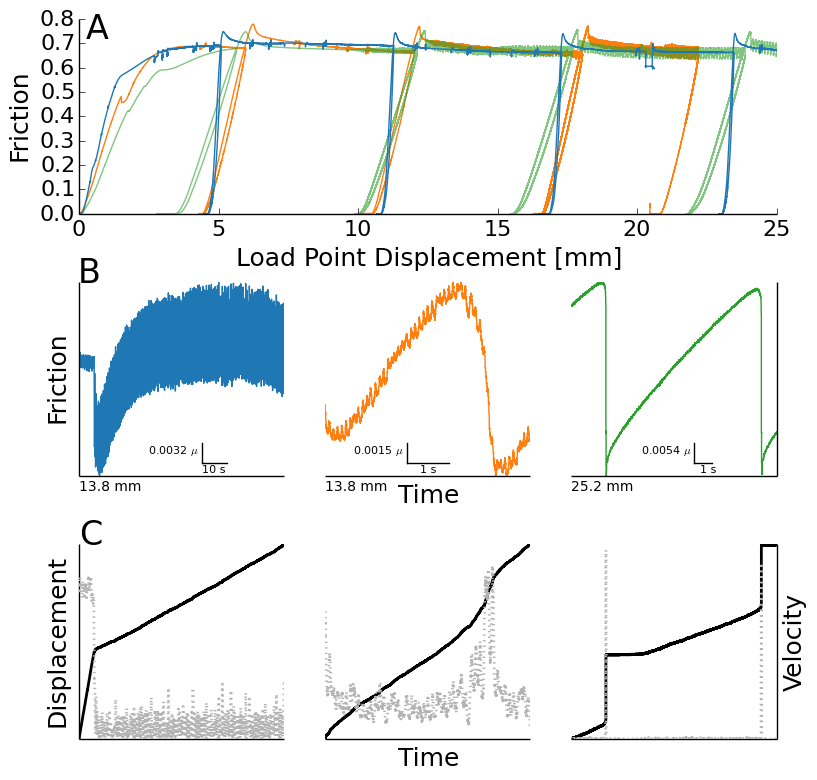
\includegraphics[scale=0.7]{../Figures/Fig_Runplot/runplot.png}
   	\caption{A) Run-plots of experiments p4309 (blue), p4311 (orange), and p4316
   	(green). Different working stiffnesses can be observed as the slope of
   	unload/reload segments. B) All steel blocks produced stable responses to
   	velocity steps (left). Destiffening the system with an acrylic center block
   	produced non-audible slow-slip events (center). Further destiffening with an
   	acrylic center block and increased normal stress produced audible fast
   	stick-slip events(right). C) Center block displacement (black) and velocity
   	(gray) for the corresponding types of failure.}
  	\label{Figure:Runplot}
\end{figure}
% End Figure %

Our observations of transitional behavior beginning when $k \sim k_c$ suggests
that $k_c$ is a valid proxy for the stability of a system, marking a transitory
zone between stable sliding and stick-slip that encompasses slow-slip and
oscillatory behavior (Fig.\ref{Figure:Stiffness Evolution}). We also observe that the critical stiffness of a system
evolves with shear strain, suggesting that tectonic faults may change behavior
as they accumulate slip and become mature fault zones.

% Figure %
\begin{figure}
    \centering
        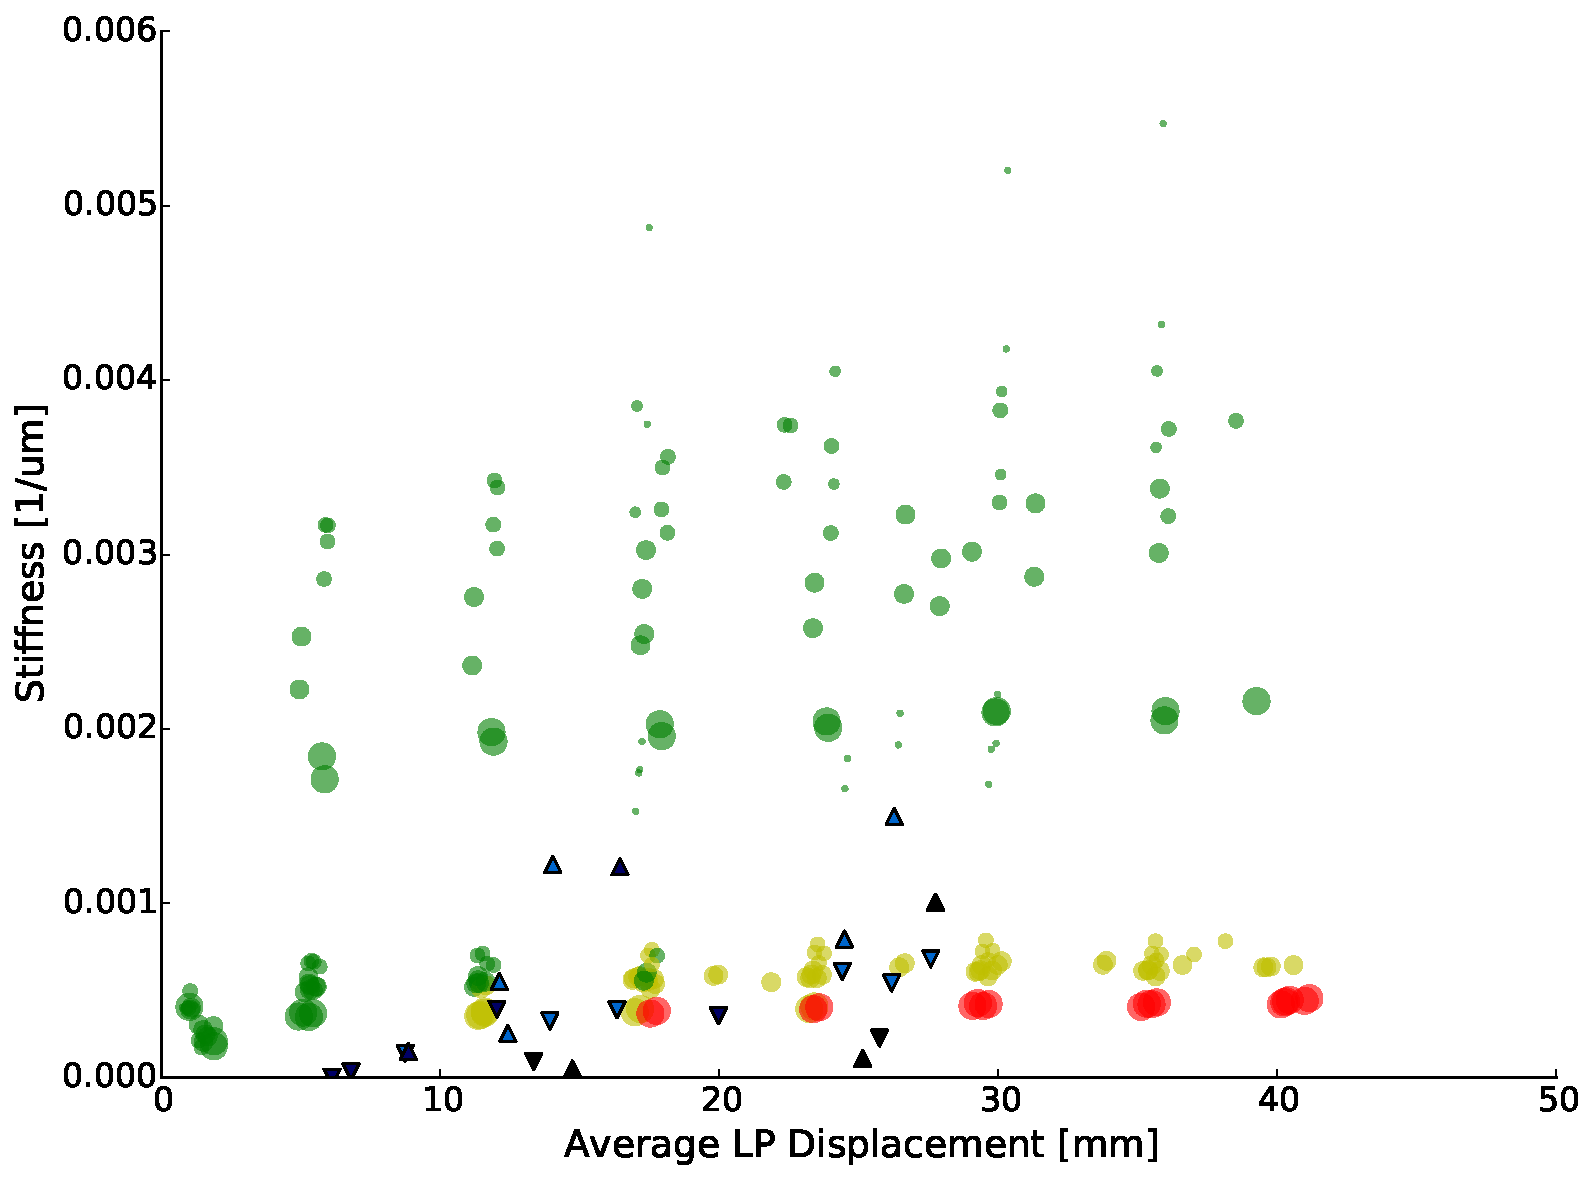
\includegraphics[scale=0.4]{../Figures/Fig_Stiffness_Evolution/Stiffness_Evolution.pdf}
       \caption{Stiffness estimates from shear stress unload/reload cycles show
       an increase in the stiffness early in shearing, likely associated with
       fabric development. Experiments with stiffness comparable to the critical stiffness
       estimates from velocity steps exhibit slow-slip behavior. Experiments in
       which the measured stiffness is below the critical stiffness exhibitied
       more rapid, audible stick-slip.}
      \label{Figure:Stiffness Evolution}
\end{figure}
% End Figure %

In nature, the critical patch size is thought of as the size a crack must grow
to before being able to support propagating dynamic rupture. Shallow VLF events in
Nankai have been shown to have critical patch sizes of $L_c = 37-63$ m,
comparable to laboratory tests on natural materials from the area
\cite{Ikari:2013}. We likewise calculate  patch sizes of 10's of meters for our
experiments, but in a simple quartz gouge,  not relying on slip dependent clay
material properties. The critical patch size (eq.\ref{equation:rc}) grows with
increasing $k_c$ and/or increasing normal stress. Extending this to large patch
sizes for slow-slip events, and assuming a nominal shear modulus ($G$), suggests
lowered normal stress and/or lowered critical stiffnesses. These arguments are
supported by inference of high pore-pressure.

% Equation - Critical Radius %
\begin{equation}
    r_c = \frac{16}{7\pi}G \frac{D_c}{\sigma_n (b-a)}
    \label{equation:rc}
\end{equation}
% End Equation %

With slow-slip failure events, we see little to no dynamic overshoot. This is observable by a period of no block motion or
deformation after the rapid stress-drop (Fig.\ref{Figure:Runplot}C).  In
traditional fast stick-slip events, the system shears further than required to
complete the force balance. Frictional oscillations and slow-slip
show no such overshoot, with continual deformation of the system throughout the
simulated seismic cycle. This provides some insight into the low frequency
nature of emissions observed from slow-slip and lack of audible report in the
laboratory. Lower shear stiffnesses will reduce the seed of rupture propagation,
softening step-like acceleration/deceleration pulses that result in high
frequency emission. Slowed rupture velocities influence disaster potential, as
tsunamogenic earthquake have generally slow rupture velocities
\cite{Kanamori:1993, Bilek:1999}.

We suggest that where in the spectrum of failure behavior a fault lies can be
quantitatively described by the relation of the stiffness of the fault compared
to the calculated critical stiffness. While factors such as pore pressure and
material frictional response are important, they are already factored into  the
stiffness comparison. We observe that the critical stiffness of a system evolves
as a fabric is developed, suggesting that accumulation of shear can change the
behavior of a fault during its lifetime.

\section{Methods}
All experiments were performed on a servo-controlled biaxial shearing apparatus.
Displacements on the normal and shearing axes were measured by Direct Current
Displacement Transducers (DCDTs) referenced at the end-platens and ram nose. The
displacement of the shearing block was measured with a DCDT referenced at the
end-platen and the top of the shearing block. Loads applied to the sample were
measured with strain gauge load cells. All transducers are semi-annually
calibrated with traceable transfer standards.

Samples were prepared in the double-direct-shear geometry using steel or
titanium side blocks and steel or acrylic shearing blocks. All blocks were
grooved 0.8 mm deep at 1 mm spacing to reduce boundary effects \cite{Anthony:2005}. The sample area
was 10 x 10 cm and filled with Min-U-Sil to a thickness of 3 mm. Granular layers
were left in a sealed container overnight with a solution of anhydrous sodium
carbonate to humidify the samples.

After samples were loaded into the load frame, a constant normal stress was
applied and maintained by the servo system in a force feedback control mode.
Samples were allowed to compact and accomodate grain rearrangement before
shearing began. Shearing is conducted at a fixed rate in displacement feedback
control mode.

Stiffness of the system was altered by changing the applied normal stress and by
changing the material of the shearing block. Increasing normal stress decreases
the effective stiffness of the system, as does switching the steel forcing block
for a cast acrylic block.

Layers were built of Min-U-Sil\textsuperscript{\textregistered} 40 fine ground
silica from the U.S. Silica\textsuperscript{\textregistered} company Berkeley
Springs, West Virginia plant. The median diameter of grain is 10.5 $\mu m$. The
product is 99.5 \% SiO$_2$, with traces of metal oxides making up the remainder.

System stiffnesses from unload/reload shear stress cycles were calculated by a
least-squares linear fit in friction vs. displacement for the interval $\mu =
0.3-0.4$. Stiffnesses from the loading portion of slow-slip and stick-slip
events were obtained with a derivative based algorithm \cite{Leeman:2015}.
Rate-and-state models were fit with both the Dieterich and
Ruina laws, with comparable results. Inversions were done with an iterative
singular value decomposition technique.

Raw data were recorded in a binary format, and can be read into Python\cite{Leeman:BiaxRead}.
Processed text output is also available

\bibliography{references}

\section{Acknowledgements}
The authors with to thank Steve Swavely for his support in the laboratory. This
material is based upon work supported by the National Science Foundation under
Grant No. DGE1255832.  Any opinions, findings, and conclusions or
recommendations expressed in this material are those of the author(s) and do not
necessarily reflect the views of the National Science Foundation. The work was
also supported by funds from the GDL Foundation and Shell Oil Company.

\section{Author Contributions}
All authors contributed to data interpretation, analysis schema, and writing.
J. Leeman conducted experiments and data analysis.

\section{Competing Financial Interests}
The authors declare no competing financial interests. Supplementary information
accompanies this paper on www.nature.com/naturegeoscience. All data is avaliable
for download, as well as Python scripts/notebooks to replicate data analysis on
GitHub (www.github.com/jrleeman). Reprints and permissions information is
available online at http://npg.nature.com/reprintsandpermissions. Correspondence
and requests for materials should be addressed to J. Leeman.

\end{document}
